\documentclass[11pt,a4paper]{article}
\usepackage[utf8]{inputenc}
\usepackage[T1]{fontenc}
\usepackage{amsmath}
\usepackage{amsfonts}
\usepackage{amssymb}
\usepackage{graphicx}
\usepackage{setspace}
\usepackage[left=2.5cm,right=2.5cm,top=2.5cm,bottom=2.5cm]{geometry}
\usepackage{float}
\usepackage[font=small,labelfont=bf]{caption}
\linespread{1.5}
\graphicspath{{./images}}

\setlength{\abovecaptionskip}{5pt}
\setlength{\belowcaptionskip}{0pt}

\begin{document}

\begin{center}
    \normalsize{Application for Admission to the PHD Programme}\\
    \textbf{\Large{A Control Framework for Morphing-Aware Navigation and Stabilization of Transformable UAVs in Constrained Environments}}\\
    \normalsize{Zilin Chen}
\end{center}

\section{Background}
\subsection{Literature Review}
The global drone industry has demonstrated remarkable growth, with market size exceeding \$30 billion in 2022 and projected to reach \$55 billion by 2030~\cite{nonami2025overview}. UAVs now serve diverse applications including precision agriculture, infrastructure inspection, and emergency response, offering unparalleled mobility and operational flexibility~\cite{COLOMINA201479}. However, their deployment in complex, constrained environments—such as agricultural greenhouses, industrial facilities, and disaster zones—presents significant challenges that conventional drone designs cannot adequately address.\\
A primary limitation of current UAV systems lies in their \textbf{fixed geometric configuration}, which restricts their ability to navigate through narrow passages and confined spaces. In agricultural applications, for instance, drones must operate within greenhouse structures where spacing between crops and support structures often falls below the minimum clearance required for standard quadrotor platforms. Similarly, inspection missions in industrial settings frequently involve traversing pipe networks, ventilation systems, and structural frameworks that demand adaptive morphology for successful penetration and navigation.\\
Transformable UAV architectures offer a promising solution to these challenges through \textbf{real-time geometric reconfiguration}. Several morphing strategies have emerged in recent research, including foldable arm designs, variable-span mechanisms, and multi-rotor topology transitions. For example, SH Derrouaoui designed a drone in a new configuration, which has rotating arms and extendable arms~\cite{derrouaoui2020dynamic}. Bin Hu also designed a new type of drone which they named as ``H 4 structure'', as it can keep the body stable when the drone's pitch changes~\cite{hu2024design}. Na Zhao designed a drone with a unique structure. The central part of the drone can be freely extended and deformed, so the arm length of the rotor drone can be easily changed~\cite{zhao2017deformable}. In addition to rotary-wing drones, researchers have also proposed deformable drones similar to fixed-wing drones. Ruben D'Sa has designed a new drone that can switch from fixed-wing to rotary-wing drone style~\cite{d2017design}. This type of drone can use solar energy to replenish energy after being unfolded, and can flexibly hover or operate when retracted into rotors. However, its limitation is that it is nearly impossible to complete mode switching during flight. Jun En Low designed another unique configuration of drone (named THOR) that can achieve the hovering of a rotary-wing drone and the cruising of a fixed-wing drone, and can also complete mode switching during flight~\cite{low2018towards}. These systems enable drones to temporarily reduce their footprint for traversing narrow spaces while maintaining optimal aerodynamic efficiency during conventional flight phases. The development of such platforms represents a significant advancement toward truly versatile aerial robots capable of operating across diverse environmental conditions.
\begin{figure}[H]
    \centering
    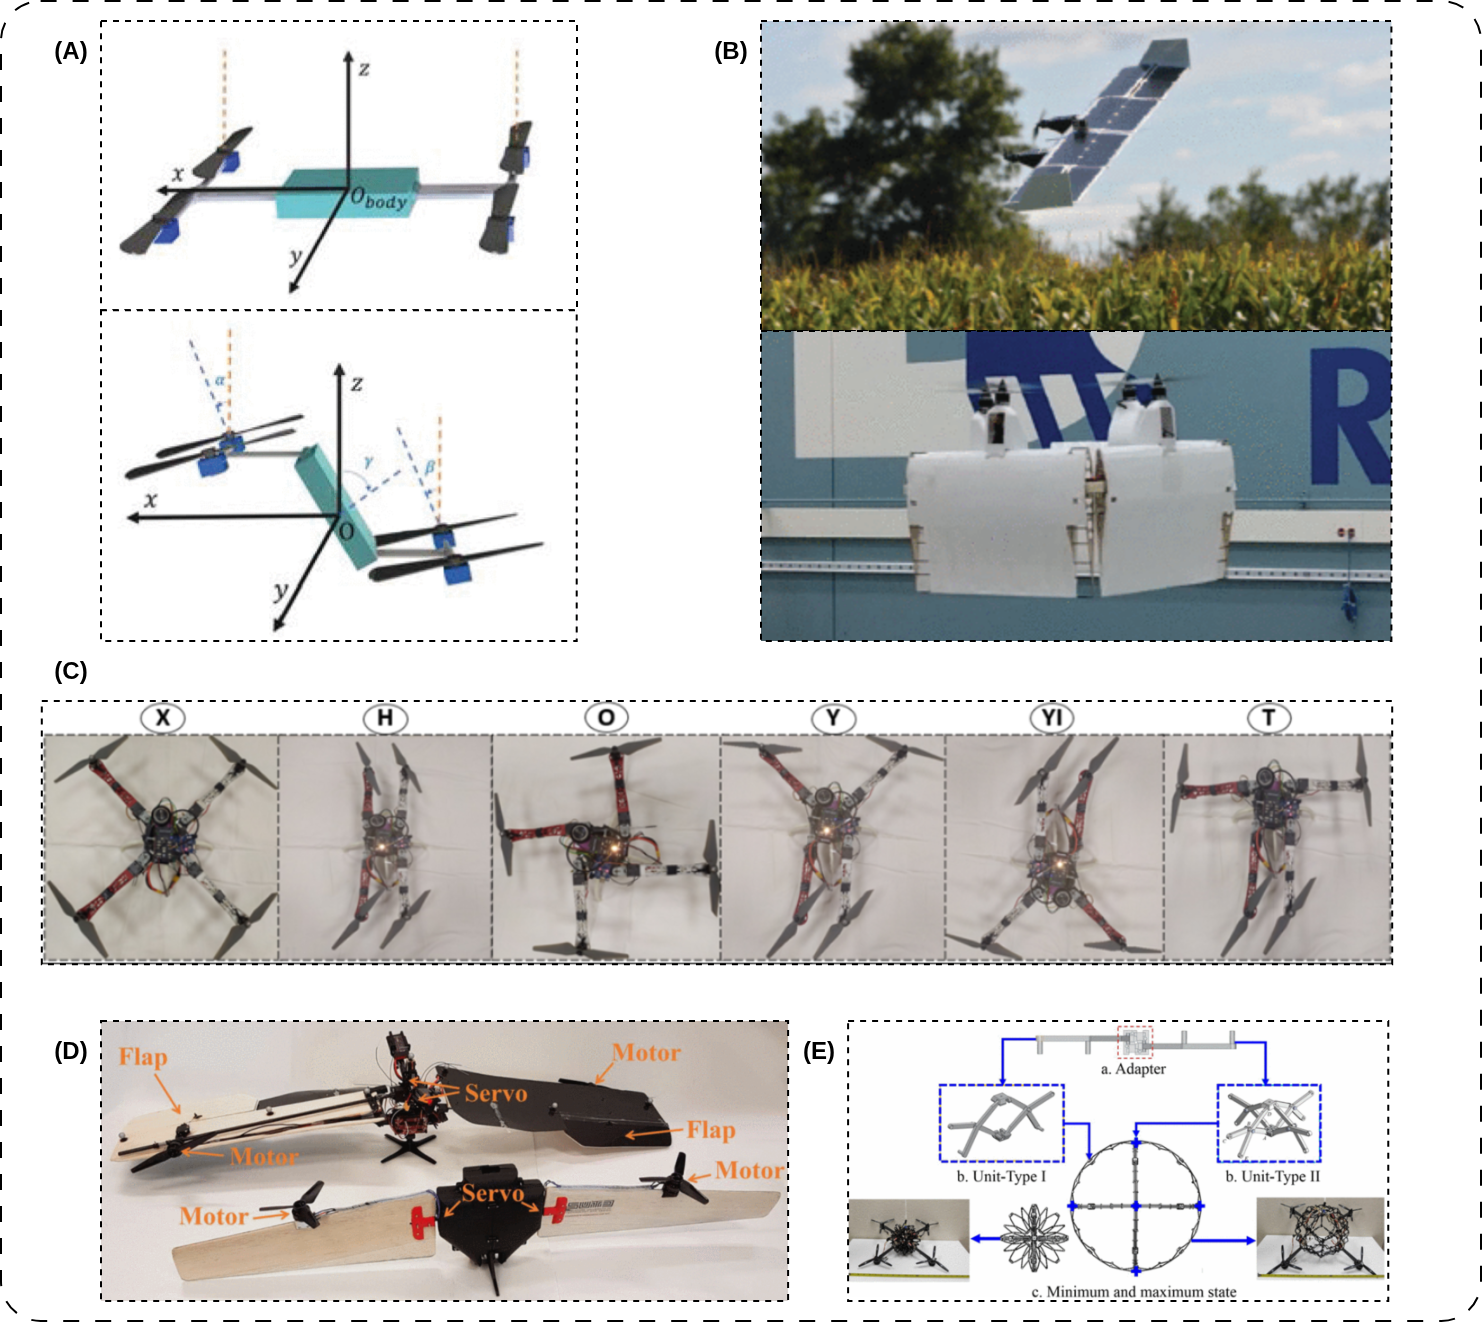
\includegraphics[width = \textwidth]{key_tech.png}
    \caption{\textbf{(A)}``H 4 structure'' quadrotor by Bin Hu.~\cite{hu2024design}\;\textbf{(B)}A drone that can switch from rotor to fixed-wing configuration and can be charged by solar energy, according to Ruben D'Sa.~\cite{d2017design}\;\textbf{(C)}SH Derrouaoui's research on a drone with variable arm length and configuration.~\cite{derrouaoui2020dynamic}\;\textbf{(D)}Jun En's THOR drone can switch between fixed-wing and rotary-wing modes during flight.~\cite{low2018towards}\;\textbf{(E)}Na Zhao's center-mounted size-adjustable drone can adapt to different usage scenarios after changing its size.~\cite{zhao2017deformable}}
\end{figure}
\noindent
Recent advances in smart materials and compliant mechanisms further enhance the potential of morphing UAVs. Shape memory alloys (SMAs), dielectric elastomer actuators (DEAs), and origami-inspired structures provide new pathways for achieving rapid, lightweight, and energy-efficient transformations~\cite{du2023high,dufour2016drone}. These technologies enable more sophisticated morphing capabilities beyond simple mechanical folding, including continuous surface deformation and multi-modal locomotion transitions.\\
The control of morphing UAVs introduces substantial complexity compared to conventional platforms. The \textbf{time-varying dynamics} resulting from geometric reconfiguration necessitate adaptive control strategies that can accommodate shifting mass properties, aerodynamic coefficients, and actuation authority. Furthermore, the integration of perception-guided morphing decisions requires tight coupling between environmental sensing and configuration management to ensure safe and efficient navigation through constrained spaces.\\
Existing flight control systems, such as the widely adopted \textbf{Betaflight} platform, provide excellent performance for fixed-geometry quadrotors but lack inherent support for morphing-aware control~\cite{betaflight}. Similarly, current planning algorithms typically assume static vehicle geometry, limiting their effectiveness for transformable platforms operating in complex environments.

\subsection{Past Experience}
During my previous research, I gained hands-on experience working with the core codebase of \textbf{Betaflight}, where I utilized its open-source platform to develop a simulator for angular velocity planning and implemented a demonstration for attitude control. I also addressed the yaw angle optimization planning problem, which has provided me with a solid background in optimization-based trajectory planning. Additionally, my practical experience with \textbf{Open-MV} and computer vision has equipped me with the skills necessary for real-time target detection and environment perception.

\section{Preliminary Design}
To enable efficient maneuverability in complex environments, this paper presents a novel transformable UAV\@. Inspired by existing mechanical designs in the literature, the drone utilizes a motor to actuate structural changes, thereby dynamically altering its arm length and moment of inertia.\\
In its default state, the distance from the drone's geometric center to the motor's geometric center is $116.59 mm$. After deformation, this distance is reduced to a minimum of $90.96 mm$, reducing the drone's size by $21.98\%$. Simultaneously, the drone's moment of inertia has significantly changed. In its default state, the principal moment of inertia along the z-axis (the direction of the motor's rotation vector) is $723,974.16 g/{mm}^2$. After deformation, it is reduced to $482,976.47 g/{mm}^2$, a $33.29\%$ reduction.
% \begin{figure}
%     \centering
%     \includegraphics[options]{name}
% \end{figure}

\section{Methodology}
This research develops and validates a hierarchical control framework for autonomous navigation of transformable UAVs in constrained environments. The methodology integrates four technical thrusts, progressing from modeling and simulation to physical validation.

\subsection{High-Fidelity System Modeling and Simulation}
This phase creates a virtual testbed that accurately captures the dynamics of the morphing UAV across its configuration space.

\subsubsection{Parameter-Varying Dynamics Modeling}
We derive a 6-degree-of-freedom nonlinear dynamic model that explicitly incorporates configuration dependent parameters, including time-varying inertia tensor, center of mass shifts, and aerodynamic coefficient variations. This model serves as the foundation for developing adaptive control strategies.

\subsubsection{Morphing Mechanism Modeling}
We develop detailed models of the transformation mechanisms, accounting for actuation dynamics, structural compliance, and aerodynamic interactions during shape transitions. Both discrete reconfiguration (e.g., foldable arms) and continuous morphing (e.g., variable geometry airframes) approaches are considered.

\subsubsection{Simulation Environment Setup}
We implement these models in \textbf{MuJoCo}, a high-performance physics simulator well-suited for complex multi-body systems with contact interactions~\cite{todorov2012mujoco}. The simulation environment includes representative constrained scenarios, such as greenhouse structures and industrial settings, to facilitate comprehensive testing and validation.

\subsection{Adaptive Control Policy Development}
The core innovation addresses the challenges of controlling a system with time-varying dynamics through a hybrid control architecture.

\subsubsection{Gain-Scheduled Flight Controller}
We design a gain-scheduled controller that adapts to the current vehicle configuration, maintaining stability and performance across the morphing continuum. Linear parameter-varying (LPV) and model predictive control (MPC) approaches are investigated for this purpose.

\subsubsection{Learning-Augmented Transition Control}
We train a \textbf{Deep Reinforcement Learning} policy to master the dynamic transitions between configurations. The policy learns to compensate for complex aerodynamic and inertial coupling effects that are difficult to model analytically.

\subsubsection{Stability-Guaranteed Recovery}
We develop control strategies that ensure rapid stabilization after completing narrow passage traversal, enabling the UAV to quickly resume efficient cruise flight in open spaces.

\subsection{Hardware Integration and Experimental Validation}
We will build a prototype to validate the simulation results in real-world conditions.

\subsubsection{Hardware Platform}
The hardware platform consists of:
\begin{itemize}
    \item A custom-built transformable quadrotor with servo-actuated morphing mechanisms.
    \item A flight controller with extended firmware supporting configuration dependent control.
    \item A perception system comprising stereo cameras and proximity sensors for environmental awareness.
\end{itemize}

\subsubsection{System Integration}
We establish a robust communication protocol between the perception, planning, and control modules. A systematic experimental evaluation measures key performance metrics:
\begin{itemize}
    \item Success rate in traversing constrained environments of varying complexity.
    \item Energy efficiency compared to conventional navigation strategies.
    \item Transition stability and recovery performance.
    \item Overall mission effectiveness in representative scenarios.
\end{itemize}

\section{Outcomes and Value}
This research delivers both theoretical advances and practical technologies that enhance UAV capabilities in constrained environments. The anticipated outcomes include:
\begin{itemize}
    \item A novel control framework for transformable UAVs that maintains stability across configuration transitions.
    \item A hardware prototype demonstrating efficient morphing and recovery in complex environments.
    \item High-fidelity simulation models and datasets reusable by the research community.
    \item Publications in top-tier robotics and autonomous systems conferences and journals.
\end{itemize}
\noindent
The successful implementation significantly expands UAV operational capabilities in applications such as precision agriculture, where drones can navigate through dense crop canopies and greenhouse structures; industrial inspection, enabling access to complex machinery and infrastructure; and search-and-rescue operations in collapsed structures. By enabling efficient navigation through constrained spaces without compromising conventional flight performance, this technology increases mission success rates and operational flexibility.\\
The primary innovation of this project lies in addressing the coupled challenge of perception, planning, and control for a system with intentionally time-varying dynamics. Unlike conventional approaches that treat morphing as a separate operational mode, our framework considers configuration as a continuous decision variable within the motion planning and control optimization. How to balance deformation stability and the benefits that deformation can bring is very important and will also be a major challenge in research.

\vspace{150pt}
\bibliographystyle{IEEEtran}
\bibliography{references}

\end{document}